%%%%%%%%%% DOCUMENT STUFF %%%%%%%%%%

\documentclass[10.5pt,letterpaper]{article}
\usepackage{mathtools}
\usepackage{amsmath}
\usepackage{amssymb}
\usepackage{datetime}
\usepackage{setspace}
\usepackage{tikz}
\usepackage[margin=1in]{geometry}
\usepackage{courier}
\usepackage{listings}
\usepackage{mips}
\usepackage{graphicx}
\usepackage{enumitem}
\usepackage{pgfplots}
\usepackage{colortbl}
\usepackage{mdframed}

%%%%%%%%%% FORMATTING %%%%%%%%%%

\newdate{date}{03}{08}{2017}
\spacing{1.5}
\date{\displaydate{date}}
\setcounter{secnumdepth}{0}
\newcommand\tab[1][0.5cm]{\hspace*{#1}}
\newcommand*\circled[1]{\tikz[baseline=(char.base)]{
            \node[shape=circle,draw,inner sep=2pt] (char) {#1};}}
\lstset{language=[mips]Assembler}
\usetikzlibrary{arrows,shapes,automata,petri,positioning,calc}

\tikzset{
    place/.style={
        circle,
        thick,
        draw=black,
        minimum size=6mm,
    },
        state/.style={
        circle,
        thick,
        draw=black!75,
        %fill=blue!20,
        minimum size=6mm,
    },
}

\graphicspath{{images/}}

%%%%%%%%%% CONTENT %%%%%%%%%%

%%%%% COVER PAGE %%%%%

\begin{document}
\title{CS 181: Homework 2}
\author{
	Jonathan Woong\\
	804205763\\
	Summer 2017\\
	Discussion 1A}
\maketitle
\pagebreak

%%%%% PROBLEMS %%%%%

\begin{enumerate}[label=\textbf{Problem \arabic*.}]
\item Minimize:
	\begin{center}
		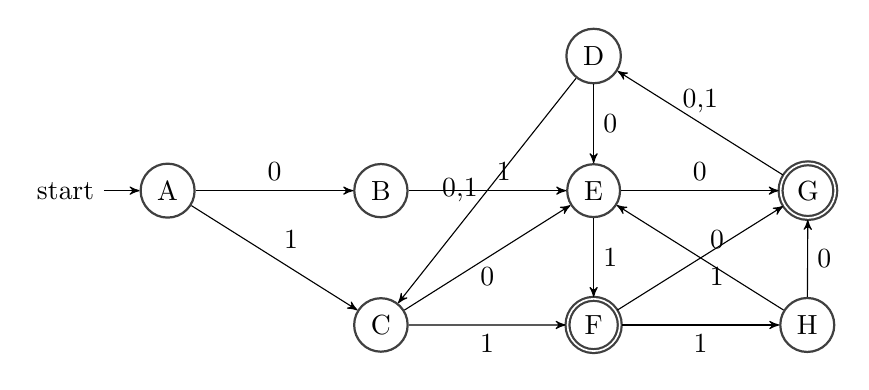
\begin{tikzpicture}[node distance=1cm and 2cm,>=stealth',auto, every place/.style={draw}]
	    \node [state,initial] (A) {A};
	    \node [state] (B) [right=of A] {B};
	    \node [state] (C) [below=of B] {C};
	    \node [state] (E) [right=of B] {E};
	    \node [state] (D) [above=of E] {D};
	    \node [state,accepting] (F) [below=of E] {F};
	    \node [state,accepting] (G) [right=of E] {G};
	    \node [state] (H) [right=of F] {H};
	    \path [->]
	    (A) edge  node {0} (B)
	    edge node {1} (C)
	    (B) edge node [left] {0,1} (E)
	    (C) edge node [below] {0} (E)
	    edge node [below] {1} (F)
	    (D) edge node [above right] {1} (C)
	    edge node {0} (E)
	    (E) edge node {1} (F)
	    edge node {0} (G)
	    (F) edge node [above right] {0} (G)
	    edge node [below] {1} (H)
	    (G) edge node [above] {0,1} (D)
	    (H) edge node [below right] {1} (E)
	    edge node [right] {0} (G);  
	\end{tikzpicture}
	\end{center}
\begin{tabular}{|c|c|c|}
\hline
\textbf{State} & \textbf{0} & \textbf{1} \\
\hline
A & B & C \\
\hline
B & E & E \\
\hline
C & E & F \\
\hline
D & E & C \\
\hline
E & G & F \\
\hline
F & G & H \\
\hline
G & D & D \\
\hline
H & G & E \\
\hline
\end{tabular}
\begin{tabular}{|c|c|c|c|c|c|c|c|c|}
\hline
TFA & \textbf{A} & \textbf{B} & \textbf{C} & \textbf{D} & \textbf{E} & \textbf{F} & \textbf{G} & \textbf{H} \\
\hline
\textbf{A} &\cellcolor{blue!25}&\cellcolor{blue!25}&\cellcolor{blue!25}&\cellcolor{blue!25}&\cellcolor{blue!25}&\cellcolor{blue!25}&\cellcolor{blue!25}&\cellcolor{blue!25}\\
\hline
\textbf{B} & X &\cellcolor{blue!25}&\cellcolor{blue!25}&\cellcolor{blue!25}&\cellcolor{blue!25}&\cellcolor{blue!25}&\cellcolor{blue!25}&\cellcolor{blue!25}\\
\hline
\textbf{C} & X & X &\cellcolor{blue!25}&\cellcolor{blue!25}&\cellcolor{blue!25}&\cellcolor{blue!25}&\cellcolor{blue!25}&\cellcolor{blue!25}\\
\hline
\textbf{D} & X & X & X &\cellcolor{blue!25}&\cellcolor{blue!25}&\cellcolor{blue!25}&\cellcolor{blue!25}&\cellcolor{blue!25}\\
\hline
\textbf{E} & X & X & X & X &\cellcolor{blue!25}&\cellcolor{blue!25}&\cellcolor{blue!25}&\cellcolor{blue!25}\\
\hline
\textbf{F} & X & X & X & X & X &\cellcolor{blue!25}&\cellcolor{blue!25}&\cellcolor{blue!25}\\
\hline
\textbf{G} & X & X & X & X & X & X &\cellcolor{blue!25}&\cellcolor{blue!25}\\
\hline
\textbf{H} & X & X & X & X & X & X & X &\cellcolor{blue!25}\\
\hline
\end{tabular}
This DFA cannot be minimized.
\item L = \{$a^nb^mc^{2(n+m)};n\geq0,m\geq0$\}\\
Find if L is:
	\begin{enumerate}[label=\alph*)]
	\item a regular language\\
	Assume that L is regular.\\
	Let $p$ = pumping length and $w = a^nb^pc^{2(n+p)} = xyz$.\\
	Suppose $n=0$ and $p=3$, then $w=b^3c^{6}=bbbcccccc=xyz$.
		\begin{enumerate}[label=\arabic*)]
		\item Let $x=b, y=bb, c=cccccc$. By pumping lemma, we expect $xy^kz \in L \ \forall k \geq 0$.\\
		Suppose $k=2$, then $w=xy^2z=bbbbbcccccc=b^5c^6 \not\in L$.
		\item Let $x=bb, y=bc, z=ccccc$. By pumping lemma, we expect $xy^kz \in L \ \forall k \geq 0$.\\
		Suppose $k=2$, then $w=xy^2z=bbbcbcccccc \not\in L$.
		\item Let $x=bbb, y=cc, z=cccc$. By pumping lemma, we expect $xy^kz \in L \ \forall k \geq 0$.\\
		Suppose $k=2$, then $w=xy^2z=bbbcccccccc=b^3c^8 \not\in L$.
		\end{enumerate}
	$\therefore$ By contradiction, L is not a regular language. We cannot build a finite automata for a non regular language.
	\item a context-free language\\
	Assume that L is context-free.\\
	Let $p$ = pumping length and $w = a^nb^pc^{2(n+p)} = uvxyz$.\\
	Suppose $n=2$ and $p=2$, then $w=a^2b^2c^8=aabbcccccccc$.
		\begin{enumerate}[label=\arabic*)]
		\item Let $u=a, v=a, x=bb, y=c, z=ccccccc$. By pumping lemma, we expect $uv^kxy^kz \in L \ \forall k \geq 0$.\\
		Suppose $k=2$, then $w=uv^2xy^2z=aaabbccccccccc=a^3b^2c^9 \not\in L$.
		\item Let $u=a, v=ab, x=b, y=c, z=ccccccc$. By pumping lemma, we expect $uv^kxy^kz \in L \ \forall k \geq 0$.\\
		Suppose $k=2$, then $w=uv^2xy^2z=aababbcccccccc \not\in L$.
		\end{enumerate}
	$\therefore$ By contradiction, L is not a context-free language. We cannot build a pushdown automata for a non context-free language.
	\end{enumerate}
\item Is any finite language regular? Prove your answer is correct.\\
Yes. A finite language L must have a finite set of strings that are accepted by L. Let these strings be denoted as $w_1,w_2,\dots,w_n$. We can express L as $w_1 \cup w_2 \cup \dots \cup w_n = \cup_{i=1}^{n}w_i$, which is a regular expression. Since any language which can be defined using a regular expression is defined to be a regular language, then by definition any finite language is regular.
\end{enumerate}
\end{document}